% !TeX root = ../main.tex
% -*- coding: utf-8 -*-

\chapter{腔磁振子系统的动力学演化}
\label{ch5}

\section{相干部分演化的解析解}
在\ref{ch4}中我们了解到了存在于腔磁振子系统中的相干竞争,因此理解系统中相干部分的行为对于分析高阶量子关联而言是一种非常有效的途径。虽然我们没办法直接求解随即微分方程组\eqref{sdes1}--\eqref{sdes4},但是如果只关注一阶量的平均还是很容易继续处理的。

我们对方程组\eqref{sdes1}--\eqref{sdes4}中的随机变量取平均值,或者直接写出一阶量$\overline{\alpha}(t)$,$\overline{\beta}(t)$的级联方程\ref{HierarchicalEq}为
\begin{equation}
\begin{aligned}
d{\overline{\alpha}}&=(-i\omega_{c}\overline{\alpha}-ig\overline{\beta}+\Omega e^{-i\omega_{0}t}-\kappa_{c}\overline{\alpha})dt \\
d{\overline{\beta}}&=(-i\omega_{m}\overline{\beta}-ig\overline{\alpha}-\kappa_{m}\overline{\beta})dt 
\end{aligned}\label{Meansdes}
\end{equation}
方程组\eqref{Meansdes}是一组含时线性微分方程组,对于一定的初始条件可以使用拉普拉斯变换来求得方程组的特解。我们这里关注更特殊的一种情况,即在初始条件为$\overline{\alpha}(0)=\mathrm{c}_0$,$\overline{\beta}(t)=\mathrm{m}_0$,驱动强度$\Omega=0$时,方程组\eqref{Meansdes}的解满足
\begin{equation}
\left(\begin{array}{c}
\overline{\alpha}(t) \\
\overline{\beta}(t)
\end{array}\right)=\left(\begin{array}{c}
\mathrm{c} \\
\mathrm{m}
\end{array}\right) e^{-i \omega t}
\label{FormalSolution}
\end{equation}
而特征向量$(\mathrm{c} \quad \mathrm{m})^T$与特征频率$\omega$满足如下的本征方程
\begin{equation}
\left(\begin{array}{cc}
\omega_{c}-i \kappa_{c} & g \\
g & \omega_{m}-i \kappa_{m}
\end{array}\right)\left(\begin{array}{c}
\mathrm{c} \\
\mathrm{m}
\end{array}\right)=\omega\left(\begin{array}{l}
\mathrm{c} \\
\mathrm{m}
\end{array}\right)
\end{equation}
可以求得两个本征频率为
\begin{equation}
\omega_{\pm}=\frac{\omega_{c}+\omega_{m}}{2}-i \frac{\kappa_{c}+\kappa_{m}}{2} \pm \sqrt{\left(\frac{\omega_{c}-\omega_{m}}{2}-i \frac{\kappa_{c}-\kappa_{m}}{2}\right)^{2}+g^{2}}
\end{equation}
因此\eqref{FormalSolution}可以进一步表示为两个本征解的线性组合
\begin{equation}
\left(\begin{array}{c}
\overline{\alpha}(t) \\
\overline{\beta}(t)
\end{array}\right)=C_{+}\left(\begin{array}{c}
\mathrm{c}_{+} \\
\mathrm{m}_{+}
\end{array}\right) e^{-i \omega_{+} t}+C_{-}\left(\begin{array}{c}
\mathrm{c}_{-} \\
\mathrm{m}_{-}
\end{array}\right) e^{-i \omega_{-} t}
\end{equation}
这里的$\left(\mathrm{c}_{\pm} \quad \mathrm{m}_{\pm}\right)^T=\frac{1}{\sqrt{\left(\omega_{\pm}-\omega_{c}\right)^{2}+\kappa_{c}^{2}+g^{2}}}\left(g \quad \omega_{\pm}-\omega_{c}+i \kappa_{c}\right)^T$,系数$C_{\pm}$由初始条件定为$C_{\pm}=\frac{\pm \mathrm{m}_{\mp}\mathrm{c}_{0}}{\mathrm{c}_{+} \mathrm{m}_{-}-\mathrm{c}_{-} \mathrm{m}_{+}}$。

在强耦合参数下$g\gg\kappa_c,\kappa_m$,光子和磁振子的相干部分可以整理为如下形式
\begin{equation}
\begin{aligned}
|\overline{\alpha}(t)|^{2} &=\left|\mathrm{c}_{0}\right|^{2}(\mathcal{A}+\mathcal{B}+2 \mathcal{C} \cos (\Delta \omega t)) e^{-2 \kappa t} \\
|\overline{\beta}(t)|^{2} &=\left|\mathrm{c}_{0}\right|^{2} \mathcal{C}(2-2 \cos (\Delta \omega t)) e^{-2 \kappa t}
\end{aligned}\label{RabiOssilation}
\end{equation}
其中$\Delta \omega=\sqrt{\left(\omega_{c}-\omega_{m}\right)+4 g^{2}}$,and $\kappa=(\kappa_{c}+\kappa_{m})/2$,而三个系数$\mathcal{A}, \mathcal{B}, \mathcal{C}$ 为 $\mathcal{A}=$ $\frac{\left|\alpha_{+} \beta_{-}\right|^{2}}{\left|\alpha_{+} \beta_{-}-\alpha_{-} \beta_{+}\right|^{2}}, \mathcal{B}=\frac{\left|\alpha_{-} \beta_{+}\right|^{2}}{\left|\alpha_{+} \beta_{-}-\alpha_{-} \beta_{+}\right|^{2}}, \mathcal{C}=\frac{\left|\alpha_{+} \alpha_{-}\right|^{2}}{\left|\alpha_{+} \beta_{-}-\alpha_{-} \beta_{+}\right|^{2}}=$ $\frac{\left|\beta_{+} \beta_{-}\right|^{2}}{\left|\alpha_{+} \beta_{-}-\alpha_{-} \beta_{+}\right|^{2}}$。

\section{连续驱动下的动力学}
这一节我们来演示使用随机微分方程模拟的方法来得到系统连续驱动下的动力学行为。在\ref{ch4}中我们得到了系统的稳态谱,但是对于腔磁振子系统如何在给定参数下从某一初始态演化为稳态的问题也是我们所感兴趣的。
\begin{figure}[htbp]
	\centering
	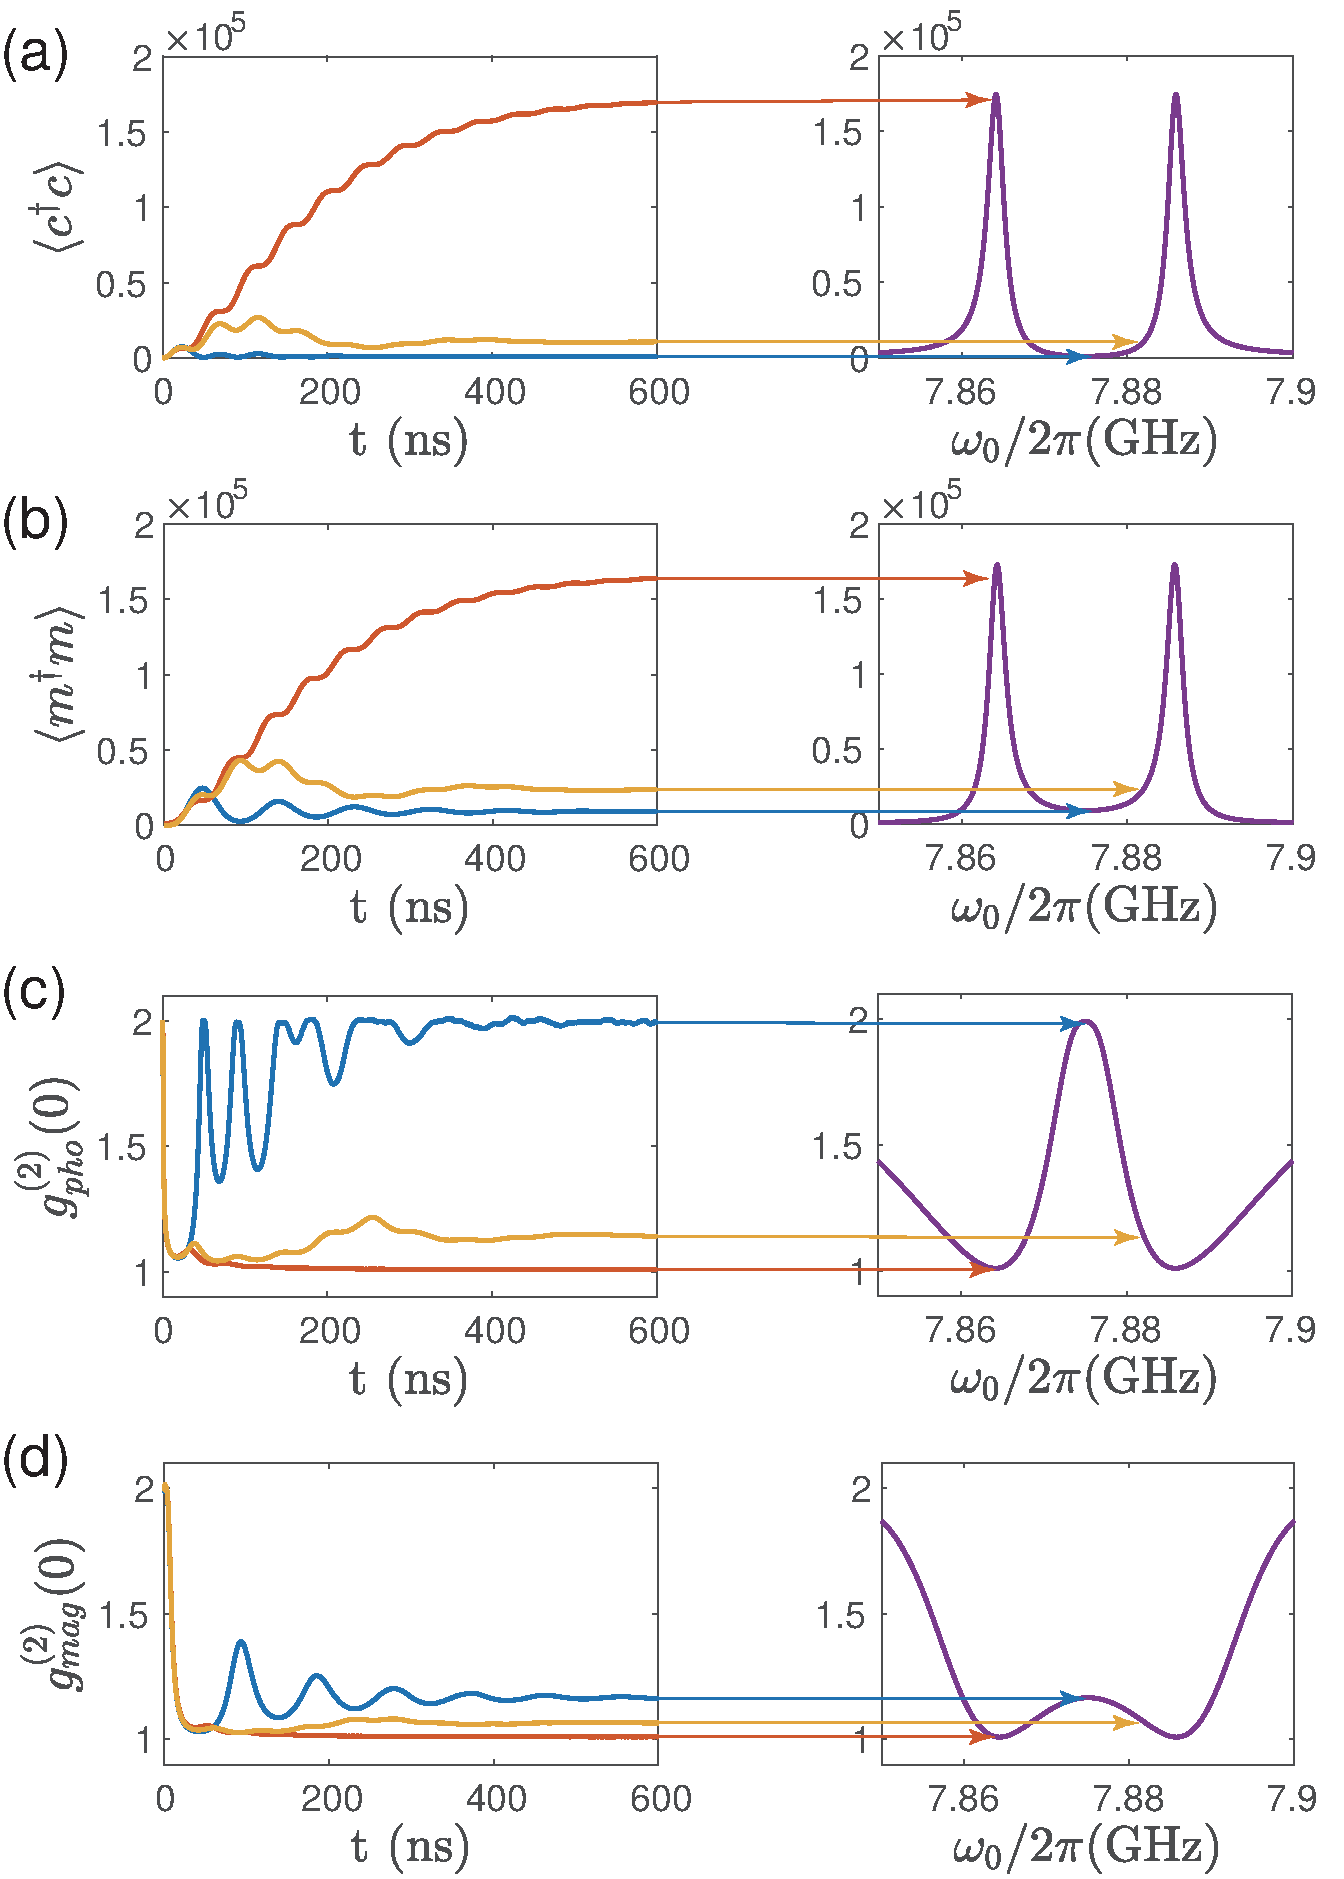
\includegraphics[width=2\basefigurewidth,clip]{./figure/5_1}
	\caption{连续驱动下平均粒子数由初态演化到稳态的过程} 
	\label{ContinuiousDrive2edOrder}
\end{figure}
我们选取强耦合下的参数:$\omega_c/2\pi=\omega_m/2\pi=7.875$ GHz, $\kappa_c/2\pi=1.35$ MHz, $\kappa_m/2\pi=1.06$ MHz, $g/2\pi=10.8$ MHz, $\Omega/2\pi=1$ GHz 以及 $T=300$ K。设置初始时刻相干的光子数与磁振数为0,随机微分方程算法的模拟步长为0.1ns,模拟样本的轨迹数量为100000。在图\ref{ContinuiousDrive2edOrder}(a)(b)(c)中我们分别模拟了400ns内$\omega_0/2\pi$取7.845GHz,7.875GHz,7.885GHz时系统中态的演化,并最终取平均计算了平均光子数$\langle c^{\dag}c(t)\rangle$和平均磁振子数$\langle m^{\dag}m(t)\rangle$。可以看到不同驱动频率下的光子和磁振子数都从0开始震荡着演化到了一个稳定值附近,而取更多个驱动频率后以稳定值和驱动频率的对应作图\ref{ContinuiousDrive2edOrder}(d),我们就重新得到了腔磁振系统平均粒子数的稳态谱线。在收敛误差内,使用这一方法所得到的稳态谱线与\ref{ch4}中的结果是完全一致的,表明了我们的级联方程方法与随即微分方程模拟的方法在理论框架内是自恰的。

\section{脉冲激励后的时间演化}
连续驱动下的计算结果作为完善我们理论的一块拼图是十分有用的,但是目前的实验并不能对这种情况下的演化行为做出测量。在微波腔系统中,实验上通常是在使用一束持续时间极短的方波脉冲驱动激励腔体之后才能对腔中光场的瞬时动力学做出测量\cite{PhysRevLett.113.156401Tang,PhysRevB.99.134445Hu}。

为了和实验对照,我们选取参数:$\omega_c/2\pi=7.875$ GHz, $\kappa_c/2\pi=1.35$ MHz, $\kappa_m/2\pi=1.06$ MHz, $g/2\pi=10.8$ MHz, $\Omega/2\pi=0$, $T=300$ K。将模拟的初态相干光子数设置为$10^8$,相干磁振子数为0,抽样次数为100000,计算不同磁场下的平均光子数时间演化如图\ref{Evolution1stOrder}(a)所示。
\begin{figure}[htbp]
	\centering
	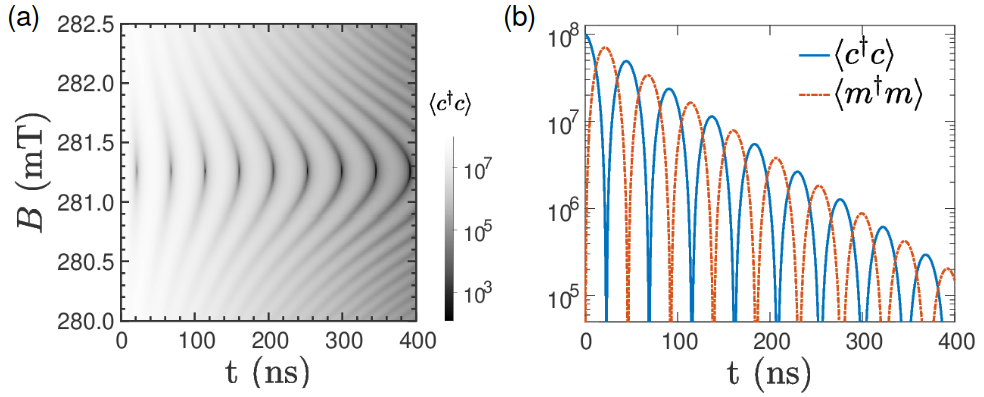
\includegraphics[width=2\basefigurewidth,clip]{./figure/5_2}
	\caption{脉冲激励后腔磁振子系统的Rabi振荡} 
	\label{Evolution1stOrder}
\end{figure}
可以看到在这种强耦合参数下,系统的瞬时动力学有着明显的振荡行为,并且随着时间的推进振荡的幅度也在一直衰减,而在磁场偏离共振的时候,由于耦合效率的降低,振荡行为也会减弱,这些特征都符合实验上的观测。为了更详细地观察系统中的振荡行为,我们取腔与磁振子共振时的磁场,把平均光子数和平均磁振子数的演化绘制在同一张图\ref{Evolution1stOrder}(b)上。我们看到腔与磁振子振荡的频率都和耦合率$g$相等,它们的相位相差$\pi$,并且振幅都随时间以相同速率指数衰减,这些行为都可以使用公式\eqref{RabiOssilation}来描述。实际上,这种表现出耦合率的振荡行为正是实现强耦合的标志之一,也就是腔QED中的Rabi振荡现象,我们这里的结果除了验证了对光场振荡行为的预测外,还证明了磁振子也有着同样的振荡行为。

虽然只靠相干部分就能理解腔磁振子系统中平均光子数和磁振子数中的Rabi振荡,但其实退相干部分的影响一直存在,我们可以从系统的二阶关联函数演化中更清晰的看到这一点。在图\ref{Evolution1stOrder}(a)的参数下,我们计算与其对应的二阶关联函数如图\ref{Evolution2edOrder}(a)所示,可以看到振荡行为此时在二阶关联函数中只出现在共振磁场的附近,偏离共振的位置处$g_{pho}^{(2)}(0)$和$g_{mag}^{(2)}(0)$都接近于1,光子和磁振子表现出极强的相干性。
\begin{figure}[htbp]
	\centering
	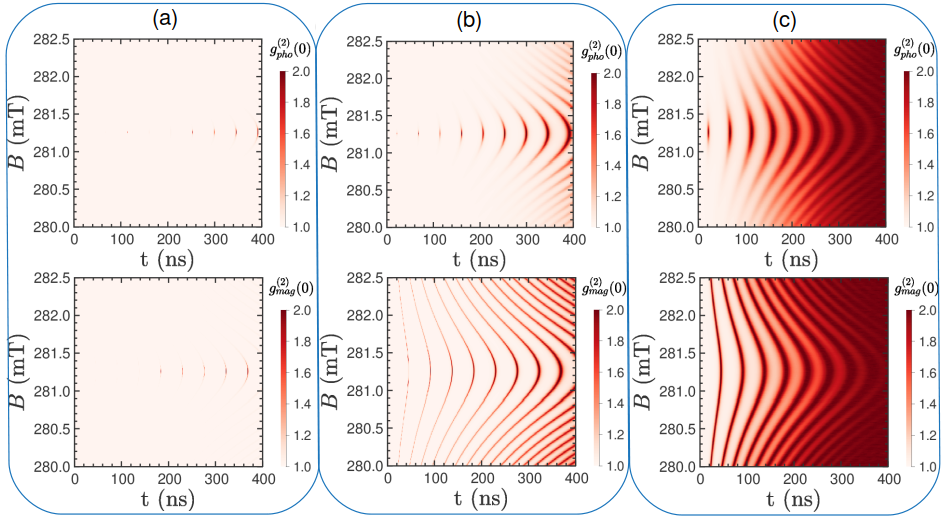
\includegraphics[width=3\basefigurewidth,clip]{./figure/5_3}
	\caption{不同初始激励下腔磁振子系统的二阶关联函数演化} 
	\label{Evolution2edOrder}
\end{figure}
与计算稳态谱时的做法类似,我们控制其他参量,依次调节初态激励的相干光子数为$10^8$,$10^6$,$10^4$,计算相应的二阶关联函数演化如图\ref{Evolution2edOrder}所示。我们同样可以看到在相干部分“退潮”的过程中,各个时刻下的非相干部分是如何显现出来的。对于相干部分与退相干部分竞争相当的图\ref{Evolution2edOrder}(b),我们再次观察到了和图\ref{Evolution1stOrder}(a)一样各处明显的振荡行为,只不过此时的振荡是光子和磁振子二阶关联函数的振荡,并且还在1与2之间变化,表明系统处于相干态和热态的频繁切换之中。另一方面,我们还可以控制温度的变化来调节非相干部分的影响。在图\ref{Evolution2edOrderTVary}中我们分别绘制了光子和磁振子共振时不同温度下系统的二阶关联函数演化,以方便更仔细地观察此时的Rabi振荡,在这里我们将初始相干光子数保持为$10^4$,其它参数和图\ref{Evolution2edOrder}(a)一致。
\begin{figure}[htbp]
	\centering
	\includegraphics[width=0.95\basefigurewidth]{./figure/5_9}
	\includegraphics[width=0.95\basefigurewidth]{./figure/5_10}
	\includegraphics[width=0.95\basefigurewidth]{./figure/5_11}
	\caption{不同温度下腔磁振子系统的二阶关联函数演化} 
	\label{Evolution2edOrderTVary}
\end{figure}
我们可以看出,在温度升高的过程中退相干部分的增强使得各个时刻的二阶关联函数都更加趋向2,表示更快地趋向于热态。虽然此时的二阶关联振荡不再表现为三角函数曲线,但是振荡频率和相位依旧和相干部分的行为一致,说明是相干部分在主导振荡的行为。

除了强耦合参数下脉冲激励后的时间演化,我们还探究了能出现MIT和Purcell效应参数下的情况。
\begin{figure}[htbp]
	\centering
	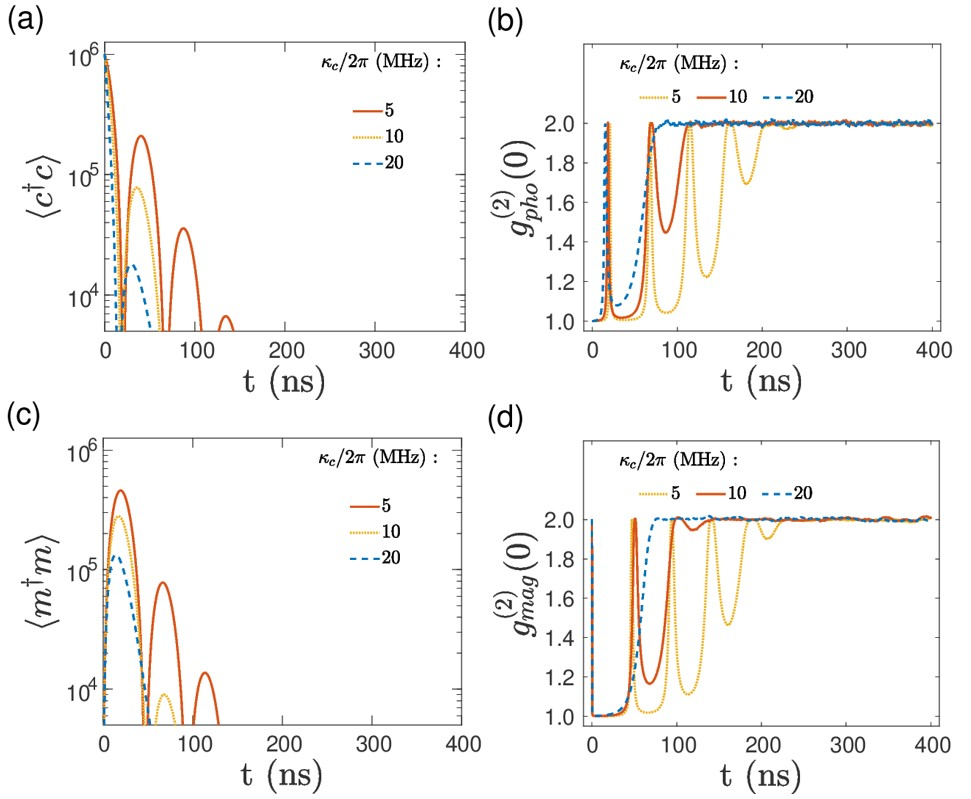
\includegraphics[width=2\basefigurewidth]{./figure/5_12}
	\caption{微腔耗散率增大时腔磁振子系统的时间演化} 
	\label{EvolutionMITKcVary}
\end{figure}
选取参数为:$\omega_c/2\pi=\omega_m/2\pi=7.875$ GHz, $\kappa_m/2\pi=1.06$ MHz, $g/2\pi=10.8$ MHz, $\Omega/2\pi=0$, $T=300$ K。在图\ref{EvolutionMITKcVary}中,我们依次取$\kappa_c/2\pi$为$5$MHz,$10$MHz,$20$MHz,计算出了对应情况下的平均粒子数以及二阶关联函数的演化行为。当$\kappa_c/2\pi=5$MHz,$10$MHz时,我们依旧能从光子和磁振子的演化曲线中看出Rabi振荡的痕迹,并且振荡的持续时间正比于$1/\kappa_c$。而当$\kappa_c/2\pi=20$MHz时,在这一耗散占主导的MIT参数下Rabi振荡的行为完全消失,初始激励的光子在很快的时间内因为耦合与耗散衰减为零,转化过来的相干磁振子又会通过耦合转换回光子,但是由于光子衰减的速率远大于磁振子的衰减速率,所以在磁振子衰减为零之后,相干光子已经全部耗散到环境之中了,最终系统中的光子和磁振子一起到达了热平衡的稳态。至于另外一个磁振子耗散占主导的情况,我们的做法类似,取$\kappa_c/2\pi=1.35$ MHz,保持其它参数和图\ref{EvolutionMITKcVary}一致,在$\kappa_m/2\pi$分别为$5$MHz,$10$MHz,$20$MHz时我们计算得到的系统演化行为如图\ref{EvolutionPurcellKmVary}所示。
\begin{figure}[htbp]
	\centering
	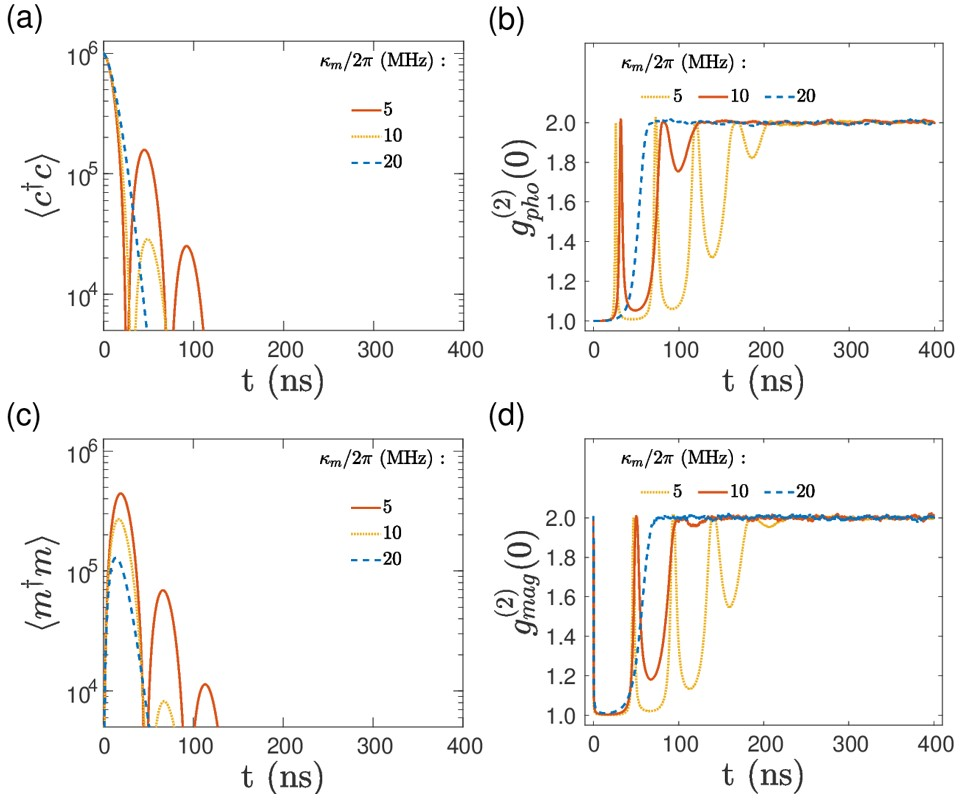
\includegraphics[width=2\basefigurewidth]{./figure/5_13}
	\caption{磁振子耗散率增大时腔磁振子系统的时间演化} 
	\label{EvolutionPurcellKmVary}
\end{figure}
同样地,我们可以看出在耗散尚未占据主导的时候,平均粒子数和二阶关联函数演化中的Rabi振荡持续时间正比于$1/\kappa_m$。而当$\kappa_m/2\pi=20$MHz时,在这Purcell效应的参数下Rabi振荡完全消失,同时由于磁振子衰减的速率反过来远大于光子的衰减速率,在磁振子获得相干能量之后就和光子一起衰减到了热稳态。在这个过程中,我们可以看出,由于与高耗散率YIG球的耦合,间接导致了光子衰减速率的增加,从\ref{EvolutionPurcellKmVary}(a)中我们可以明显看出光子的指数衰减速率要大于$\kappa_c/2\pi=1.35$ MHz,单看这一条衰减曲线就仿佛光子的耗散率增大了一样,这也正是Purcell效应在时间演化中的体现。
